\documentclass[english]{article}
\usepackage[T1]{fontenc}
\usepackage[latin9]{inputenc}
\usepackage{listings}
\usepackage{amsmath}
\usepackage{graphicx}
\usepackage{babel}
\begin{document}

\subsection*{The Wishart Distribution}


\subsection*{The Bartlett Decomposition}

Under a given variance matrix $V$, the Bartlett Decomposition is
the equation.

\begin{align*}
\mathbf{W} & =\Gamma^{T}A^{T}A\Gamma
\end{align*}
in the context that $\Gamma$ is the upper triangular part of the
Cholesky decomposition

\begin{align*}
V= & \Gamma^{T}\Gamma
\end{align*}


and $A$ is a $d\times d$ matrix with entries defined by the \textbf{independent
}random variables

\begin{align*}
\mathbf{A_{\text{row},\text{column}}}\sim & \begin{cases}
0 & \text{row}>\text{column}\\
\chi_{\text{df}-(\text{row}-1)}^{2} & \text{row}=\text{column}\\
N(0,1) & \text{row}<\text{column}
\end{cases}
\end{align*}


which is upper triangular since everything below the diagonal is 0.
All this means that  $\mathbf{W}$ is Wishart-distributed with $df$
``degrees of freedom'':

\begin{align*}
\mathbf{W} & \sim W(\Gamma^{T}\Gamma,df)
\end{align*}


~

Note that the Bartlett decomposition is also the LU decomposition
of $\mathbf{W}$, since the form of the terms in $\mathbf{W}=\Gamma^{T}A^{T}A\Gamma$
is ``LLUU'', the product of two lower (or upper) triangular matrices
is lower (or upper) triangular and the LU decomposition, if it exists,
is unique.

~

This theorem has a couple of equivalent forms (Wikipedia  for example,
defines $\mathbf{W}=\Gamma AA^{T}\Gamma^{T}$, or you could also start
from the theorem that $A^{T}A\sim W(I,df)$ and then prove that Wisharts
can be scaled: $M\sim W(V,df)\wedge(C\text{ is invertible and square})\implies CMC^{T}\sim W(CVC^{T},df)$
). We choose this form because the value of $chol()$ in most libraries
(certainly, in R) is an \textbf{upper triangular matrix} and following
that lead clarifies our derivations and the programs built on them.


\subsection*{Generating Wishart Variates}

This decomposition actually gives a useful way to \emph{generate }a
desired Wishart distribution: if you want to generate not-quite-covariance
Wishart matrices and you know (or think you know) $V$ and $df$,
you sample $A$ according to the rule above (using $df$), find $\Gamma\leftarrow chol(V)$,
scale $A$ by $U\leftarrow A\Gamma$, and square that: $\mathbf{W}\leftarrow U^{T}U$.
The only stochastic part is the generation of $A$.


\subsubsection*{Runtimes}

We traced R's ```rWishart.c``` and worked out that it uses precisely
this algorithm. Translating that R/C/Fortran mixture into pseudocode:

\begin{lstlisting}
def std_bartlett_factor(d, df): #named std_rWishart_factor in the C
  A = matrix(d,d)
  for i in [0 to d-1]:  #note that the matrices are 0-indexed here
    A[i,i] = sqrt(rchisq(df - i)) #generate X^2_df-(row-1) variates
    for j in [j+1 to d-1]: #TODO: (d-1 - j+1) = how many elements?
      A[i,j] = rnorm()            #generate N(0,1) 
      
  return A
  
def rWishart(n, df, V):
  d = dim(V)[0]
  assert d == dim(V)[1], "Psi must be square"
  #Unchecked: Psi must be positive definite
  
  gamma = chol(V) #(cache the upper triangular cholesky factor) #lines [...]
  V = new matrix(d,d,n)
  for k in [1 to n]:   #(loop to take samples)
    A = std_bartlett_factor(d, df) #sample A
    U = A*gamma           #scale the sample
    V[n] = U'*U           #construct V
  return V
\end{lstlisting}


std\_Wishart\_factor takes $O(\frac{d(d+1)}{2})=O(d^{2})$ time, since
it has to operate on half the matrix. From Wikipedia  $chol()$ takes
$d^{2}/3$ time. Matrix multiplication, in general, takes $O(d^{3})$
time but the authors of this code use specialized Fortran BLAS routines
that shorten this slightly to exploit a) the upper triangularness
of U b) the symmetry of U'U so that the first matrix multiply only
takes {[}...{]} and the secondtakes {[}...{]}..

The routine for a) is called dtrmm.f and the relevant section of its
code is

\begin{lstlisting}
              IF (UPPER) THEN
                  DO 180 J = N,1,-1
                      TEMP = ALPHA
                      IF (NOUNIT) TEMP = TEMP*A(J,J)
                      DO 150 I = 1,M
                          B(I,J) = TEMP*B(I,J)
  150                 CONTINUE
                      DO 170 K = 1,J - 1
                          IF (A(K,J).NE.ZERO) THEN
                              TEMP = ALPHA*A(K,J)
                              DO 160 I = 1,M
                                  B(I,J) = B(I,J) + TEMP*B(I,K)
  160                         CONTINUE
                          END IF
  170                 CONTINUE
  180             CONTINUE
\end{lstlisting}


In our case, $N=M=d$, so if you squint this says ``in a d-length
loop with itertor j do (a d-length loop and a j{*}d length loop)'',
which means $O(d\cdot(d+\sum_{j=1}^{d}j))=O(d\cdot(d+\frac{d(d+1)}{2}))=O(d^{2}+\frac{d^{3}+d^{2}}{2})=O(\frac{d^{3}+3d^{2}}{2})=O(d^{3})$
and the structure of dsyrk is almost identical  and then there's
an extra $\frac{d(d+1)}{2}$ loop in the C code to fill in the symmetric
half of the matrix that dsyrk doesn't do.

I won't count the time for memory allocation because that is much
more dependent how on the $malloc$ in use, how fragmented RAM is,
whether a cache is involved, and whether $d^{2}>\text{\ensuremath{malloc}page size}$.
Adding this all up, we see that run time of rWishart is $O(1)+d^{2}/3+n\cdot(O(\frac{d^{3}+3d^{2}}{2})+O(\frac{d^{3}+3d^{2}}{2}+\frac{d(d+1)}{2}))=O(d^{2}/3+n\cdot(d^{3}+3d^{2}+\frac{d(d+1)}{2}))=O(n\cdot d^{3}+3(n+\frac{1}{3})d^{2}))=O(n\cdot d^{3})$.

~

The consequence of this is that is that doubling the number of variates
$d$ in your model will extend your runtime by eight. So, a sampler
that runs on the order of minutes would run, on double the variates,
in tens of minutes, and a sampler than runs in tens of minutes will
take hours. Further, techniques like bootstrap sampling generally
want $n$>\textcompwordmark{}>$d$, so in practice runtime is $O(d^{4})$
or higher. 




\subsection*{The Inverse Wishart Distribution}

The inverse Wishart distribution shows up when trying. It gives \emph{precision
matrices} instead of \emph{variance matrices} .


\subsection*{Generating Inverse Wishart Variates}

The naive algorithm for generating inverse wisharts is:

\begin{lstlisting}
def rInvWishart(n, df, P):  #P for "precision"
  V = invert(P)
  return [invert(W) for W in rWishart(n, df, V)]
\end{lstlisting}


With identical runtime to $rWishart$ plus $n+1$ extra inversion
operations. According to Wikipedia,  matrix inversion takes between
$O(d^{2.3})$ and $O(d^{3})$. So the total runtime is in $O(n\cdot d^{3})+(n+1)\cdot O(d^{3})=O((2n+1)\cdot d^{3})$,
or roughly twice as slow as $rWishart$. This is also dangerous because
raw $invert()$ is the most numerically unstable operation around.\\
~

ALSO . triangular-solve (aka backsolve) takes O(d\textasciicircum{}???)
per column

and triangular-multiply is O(d\textasciicircum{}2)

and triangular-inverse (a special case of backsolve) takes O(d\textasciicircum{}??)



~

But we can do better (and when we get to the Normal-InverseWishart,
the same trick we use here will give us extra speedups there).

~

Let's take a look at what $invert(W)$ \textbf{\emph{is}}. 

\begin{align*}
\mathbf{W} & =\Gamma^{T}A^{T}A\Gamma\\
 & =U^{T}U\\
\mathbf{W}^{-1} & =\Gamma^{-1}A^{-1}\left(A^{-1}\right)^{T}\left(\Gamma^{-1}\right)^{T} & \text{invert swaps order, and is swappable with transpose}\\
 & =\Gamma^{-1}A^{-1}\left(\Gamma^{-1}A^{-1}\right)^{T} & \text{transpose swaps order, too}\\
 & =U^{-1}\left(U^{-1}\right)^{T}\\
U^{-1} & =\Gamma^{-1}A^{-1}
\end{align*}


Now, recall what $\Gamma$ is: $chol(V)=chol(P^{-1})$

\begin{align*}
U^{-1} & =\Gamma^{-1}A^{-1}\\
 & =chol(P^{-1})^{-1}A^{-1}\\
\end{align*}


With $chol(P^{-1})$ and $A^{-1}$ both upper triangular, which is important because a) we can compute $U^{-1}$ with backsolve b) $U^{-1}$ is upper triangular itself. Unfortunately, there is no clever way around computing $P^{-1}$ directly, but it can be precomputed at the start so it does not eat into the runtime of the overall algorithm.

We care about this $U$ it lets us get samples $V$ and $X$:

\begin{align*}
V & =U^{-1}\left(U^{-1}\right)^{T}\\
\\
X & =\mu+U^{-1}z & \text{where }z\sim N_{d}(0,I)\\
 & =\mu+chol(P)A^{-1}z\\
 & =\mu+\Gamma^{-1}A^{-1}z
\end{align*}


\subsubsection*{Runtime of Full Matrix Multiplication}

\begin{align*}
\sum_{i=1}^{d}\sum_{j=1}^{d}2(d)-1= & \sum_{i=1}^{d}d(2d-1)\\
= & d^{2}(2d-1)
\end{align*}



\subsubsection*{Runtime of Triangular Matrix Multiplication}

A triangular matrix by a triangular matrix (of the same sidedness)
can be sped up a bit over the full multiply.

Suppose our matrices are lower triangular.

As before, the value of each entry in the result matrix $S$ is$S_{ij}=\sum_{k=1}^{d}A_{ik}B_{kj}$.

Since our matrices are lower triangular, they have the property that
$A_{cd}=0$ if $c<d$ (everything with row strictly above column is
null). This has two consequences:

1) the terms in $S_{ij}=\sum_{k=1}^{d}A_{ik}B_{kj}$ are $0$ if $i<k$
or $k<j$ since at least one of $A_{ik}$ and $B_{kj}$ are zero in
that case. That is, for $k\in[1,d]$, the only nonzero terms are $k\in[1,d]\setminus(i,d]\setminus[1,j)$=.
So if we are told our matrices are lower triangular, we know without
looking that we can shorten innermost loop to:

$S_{ij}=\sum_{k=j}^{i}A_{ik}B_{kj}$ which has one multiply for each
term in the sum and one add (less one) for each, giving runtime:

$(i-j+1)+(i-j+1)-1=2(i-j)+1$

2) $[j,i]=\emptyset$ if $i<j$, so $S_{ij}=0$ in that case, meaning
that the output matrix is again lower triangular, and we can skip
doing any work at all in that case: we only need to send our second-inner
loop from 1 to i, not 1 to d.

If our matrices are instead uppertriangular, notice that $AB=(AB)^{T^{T}}=(B^{T}A^{T})^{T}$,
which is the transpose of the product of two lower triangular matrices.
Transposing is constant time (in a wise implementation) and only $d^{2}$
time elsewhere, so this algorithm holds in either case.

However, with

\begin{align*}
\sum_{i=1}^{d}\sum_{j=1}^{i}2(i-j)+1= & \sum_{i=1}^{d}i\cdot(2i+1)-\sum_{j=1}^{i}2j\\
= & \sum_{i=1}^{d}i\cdot(2i+1)-2\frac{i(i+1)}{2}\\
= & \sum_{i=1}^{d}i\cdot(2i+1-(i+1))\\
= & \sum_{i=1}^{d}i\cdot((2-1)i+(1-1))\\
= & \sum_{i=1}^{d}i^{2}\\
= & \frac{1}{6}d(d+1)(2d+1)
\end{align*}


Full multiply has leading term $2d^{3}$, while this has leading term
$2d^{3}/6$. So this algorithm is about six times faster than naive,
full, dense matrix multiplication. This doesn't crack this algorithmic
nut, \textbf{but it could make the difficult possible}.


%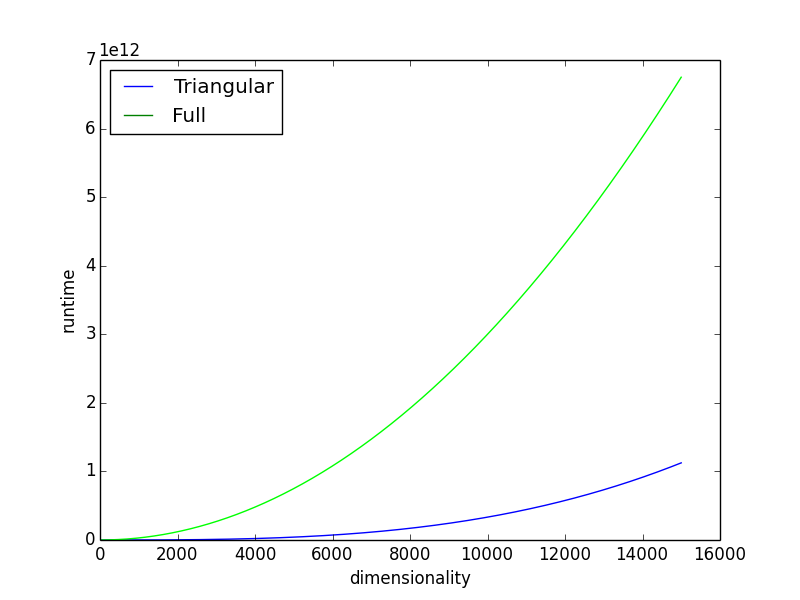
\includegraphics[scale=0.7]{full_vs_triangular}


\section*{Lemmas}

\subsection*{chol(P)}

\subsection*{Inverse of a triangular matrix}

Suppose $T$ is a triangular matrix (lower or upper). Then $T^{-1}$ is also triangular (lower or upper, respectively).

Proof:


\begin{align*}
T T^{-1} &= I \\
\end{align*}


$T^{-1} = backsolve(T, I)$

so column $i$ of $T^{-1}$ is
 $backsolve(T, [0 ... 1 ... 0 0 0 0 ... 0]^T) $
 with the 1 in the $i$th position.

so ... ?

\section*{The Matrix Normal Dist}


the matrix normal can also be thought as a single multivariate normal $N(vec(\mu), V \otimes K)$
but this loses some of the structure intrinsic to it

this identity is relevant to this: $sqrt(V \otimes K) vec(X) = vec(K X V)$
note that $K \cdot X \cdot V ~ MN(0, K, V)$ if $X$ is a $q \times p$ matrix of i.i.d. standard normals.

You can view the matrix normal as a set of multivariate normals: down the columns you have variance (as in a single multivariate normal)
 and then by doing some transposes (TODO: work out this derivation) you can again cross the columns.

\section*{Identities}

The scatter matrix
$S = (X^TX)$
can be rewritten (and viewed) as the sum of (outerproduct) squares
$S = \sum_{i=1}^n (x_i - \bar(x))(x_i - \bar(x_i))^T$

where $x_i$ are the rows of X

$tr(V^{-1} S) = \sum_{i=1}^n mahalanobis(x_i, E(x_i), V)$
Proof: 
. ...

\end{document}
